\documentclass[12pt,a4paper]{article}

\usepackage[pdftex]{graphicx}
%\usepackage{cite}
\usepackage{indentfirst}
\setlength{\parindent}{1em}
\usepackage{enumerate}
\usepackage{geometry}
\geometry{left=1in,right=1in,top=1in,bottom=1in}
%\usepackage{times}
%\usepackage{mathptmx}
%\usepackage{listings}
%\usepackage[framed,numbered,autolinebreaks,useliterate]{mcode}
\usepackage{amsmath}
\usepackage{amssymb}
\usepackage{tcolorbox}

%\title{Vision Control - final project}
\title{Lyapunov based Nonlinear Control - final project \\ [2ex] \begin{large} Adaptive Vision-Based Leader-Follower \\ Formation Control of Mobile Robots \end{large} }
\author{Sun Qinxuan}

\begin{document}
\maketitle

\section{Paper Overview}

\indent An adaptive controller is proposed for a vision-based leader-follower formation control of mobile robots. The adaptive controller proposed does not require the knowledge of camera's intrinsic and extrinsic parameters, and also the relative position measurement and communication between the leader and follower. A real-time observer is developed to estimate the unknown parameters in the system. And the Lyapunov method is employed to prove the stability of the closed-loop system to guarantee the convergence of the image error.

\begin{figure}
  \centering
  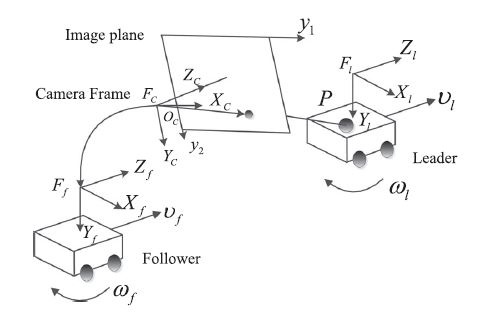
\includegraphics[width=0.5\textwidth]{figs/model.jpg}% 1\linewidth
  \caption{Schematic pipeline of CPA-SLAM system.}
  \label{model}
\end{figure}

\section{Method Description}


\subsection{Problem Statement}

\indent The coordinate frames are illustrated in Figure \ref{model}. The robot's linear velocity is defined along its $Z$-axis, and its angular velocity is orthogonal to the ground plane. The follower, leader, camera and feature point are denoted by the letters $f$, $l$, $C$ and $P$, respectively. The presuperscript represents the frame that the variable is relative to. For instance, ${}^fx_P$ denotes the coordinate of the feature point $P$ along $X_f$ axis.

\indent Given a desired position ${\bf y}_d$ defined on the image plane of the follower robot and let the feature point $P$ on the leader robot be in the field of view of the follower's camera. The objective is to design a kinematic controller to position the follower robot such that the feature point $P$ is guaranteed to converge asymptotically to an arbitrarily small circle around the desired position.

\subsection{Kinematics}

\indent The 3D coordinates of feature point $P$ relative to $F_f$ is denoted by ${}^f{\bf P}_P$. And $\gamma$ denotes the relative orientation and $\bf n$ denotes the 3D coordinates of the feature point $P$ relative to $F_l$. The system has two independent inputs, the linear velocity $v_i$ along axis $Z_i$ and the angular velocity $\omega_i$ along axis $Y_i$. Let ${\bf u}_i=[v_i,\omega_i]^T$.
\begin{equation}
{}^f\dot{\bf P}_P={\bf J}_{ff}({}^f{\bf P}_P){\bf u}_f+{\bf J}_{lf}({\bf n},\gamma){\bf u}_l,\
\dot \gamma = \omega_l-\omega_f,
\end{equation}
where
\begin{equation}
{\bf J}_{ff}=
\left[
\begin{array}{cc}
    0  &-{}^fz_P \\
    0  &0 \\
    -1 &{}^fx_P \\
\end{array}
\right]
\end{equation}
\begin{equation}
{\bf J}_{lf}=
\left[
\begin{array}{cc}
    \sin\gamma  &-n_x\sin\gamma+n_z\cos\gamma \\
    0           &0 \\
    \cos\gamma  &-n_z\sin\gamma-n_x\cos\gamma \\
\end{array}
\right]
\end{equation}

\indent Let ${}^C{\bf P}_P$ denote the 3D coordinates of $P$ with respect to $F_C$. Then,
\begin{equation}
\left[
    \begin{array}{c}
    {}^C{\bf P}_P \\
    1
    \end{array}
\right]
=\left({}^f{\bf g}_C\right)^{-1}
\left[
    \begin{array}{c}
    {}^f{\bf P}_P \\
    1
    \end{array}
\right]
\end{equation}
Taking the time derivative and substituting for ${}^f\dot{\bf P}_P$ results in
\begin{equation}
{}^C\dot{\bf P}_P={\bf J}_{fC}({}^C{\bf P}_P){\bf u}_f+{\bf J}_{lC}(\gamma){\bf u}_l.
\label{cpp}
\end{equation}

The projection of $P$ on the image plane is denoted by
\begin{equation}
\left[
    \begin{array}{c}
    {\bf y}\\
    1
    \end{array}
\right]
=\frac{1}{{}^Cz_P}{\bf A}{}^C{\bf P}_P,
\label{y}
\end{equation}
where ${\bf y}=[y_1,y_2]^T$ and ${\bf A}$ is the intrinsic matrix of the camera. Combining (\ref{cpp}) and (\ref{y}) results in
\begin{equation}
\dot{\bf y}={\bf J}_{fy}({}^C{\bf z}_P^{-1},{\bf y}){\bf u}_f+{\bf J}_{ly}({}^C{\bf z}_P^{-1},\gamma){\bf u}_l.
\end{equation}
Suppose that the feature point $P$ moves on a fixed plane, the plane equation can be exploited to remove the unknown depth ${}^C{\bf z}_P$, yielding
\begin{equation}
\dot{\bf y}={\bf H}({\bf t}){\bf u}_f+{\bf G}(\gamma){\bf u}_l={\bf H}({\bf t}){\bf u}_f+{\bf F}(\gamma,v_l,\omega_l).
\label{doty}
\end{equation}

\indent There is a property here. For any 2D vector ${\bf u}=[v\ \omega]^T$, ${\bf H}(\theta, {\bf y}){\bf u}$ and ${\bf \dot H}(\theta, {\bf y, \dot y}){\bf u}$ can be parameterized in the following linear form
\begin{equation}
{\bf H}(\theta,{\bf y}){\bf u}={\bf M(y,u)}\theta,\ 
{\bf \dot H}(\theta,{\bf y, \dot y}){\bf u}={\bf N(y,\dot y ,u)}\theta
\end{equation}
where $\theta \in {\mathfrak R}^{16\times1}$ denotes all the constant unknown parameters.

\begin{figure}
  \centering
  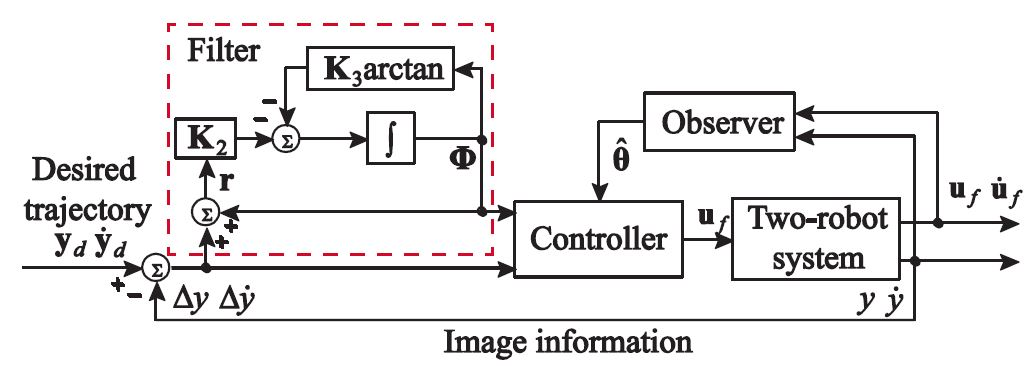
\includegraphics[width=0.6\textwidth]{figs/control.jpg}% 1\linewidth
  \caption{Control block diagram.}
  \label{control}
\end{figure}


\subsection{Adaptive Vision-based Formation Control}

\indent The control block diagram is shown in Figure \ref{control}. The image-based error containing the image position error and the image velocity error are exploited as the feedback signal. And a filter is designed to generate an image-based signal to compensate for the absence of the unknown matrix $\bf F$.

\indent The image-based error $\bf r$ is defined as
\begin{equation}
{\bf r}=\bf s\Delta \dot y +k\Delta y+\Phi
\end{equation}
where $ {\bf\Delta y}=[y_1-y_{1d}\ y_2-y_{2d}]^T$ and ${\bf\Delta \dot y}=[\dot y_1 \ \dot y_2]^T$. The signal generated by an image-based filter is given by ${\bf \Phi}=[\Phi_1\  \Phi_2]^T$. And the image-based filter is designed as
\begin{equation}
\dot{\bf \Phi }=-{\bf K}_3{\bf \Psi}-{\bf K}_2{\bf r},\quad {\bf \Phi}(0)={\bf 0}_{2\times1}
\end{equation}
where ${\bf \Psi}=[\arctan\Phi_1\ \arctan\Phi_2]^T$ and $\bf s, k, K_2, K_3$ are positive definite and diagonal gain matrices. The differential of the image-based error is $\bf \dot r=s\Delta \ddot y+k\Delta\dot y+\dot\Phi$. Substituting (\ref{doty}) into it yields
\begin{equation}
\dot {\bf r}={\bf sH\dot u}_f+({\bf s\dot H +kH}){\bf u}_f+\bf s\dot F+kF-K_3 \Psi-K_2 r
\end{equation}



\indent The following controller is proposed
\begin{equation}
\dot{\bf u}_f=({\bf s\hat H})^{-1}
\left(
-{\bf K}_1{\bf r}+{\bf \Gamma}^{-1}_1{\bf K}_2{\bf \Pi}+{\bf K}_3{\bf \Psi}
-\left({\bf s\hat{\dot H}+k\hat H}\right){\bf u}_f-{\bf K}_4\left\|\frac{\partial U}{\partial \hat \theta}t\right\|{\bf r}
\right)
\end{equation}

\indent To estimate the unknown parameters in the controller, the observer is designed as follows
\begin{equation}
\dot{\hat \theta}={\bf\Gamma}^{-1}_2
\left[
\left(
{\bf M}^T({\bf y,\dot u}_f){\bf s}+{\bf N}^T({\bf y,\dot y,u}_f){\bf s}+{\bf M}^T({\bf y,\dot u}_f){\bf k}
\right)
{\bf \Gamma}_1{\bf r}+{\bf r}^T{\bf r K}_5\frac{\partial U}{\partial \hat \theta}
\right]
\end{equation}
To analyze the system stability, introduce the following Lyapunov function
\begin{equation}
V=\frac{1}{2}{\bf r}^T{\bf\Gamma}_1{\bf r}+{\bf L}^T{\bf \Lambda L}
+\frac{1}{2}{\tilde\theta}^T{\bf\Gamma}_2{\tilde \theta}+\frac{1}{2}\gamma^2.
\end{equation}
$V$ can be considered as two parts, $V_1$ and $V_2$.
\begin{equation}
V_1=\frac{1}{2}{\bf r}^T{\bf\Gamma}_1{\bf r}+{\bf L}^T{\bf \Lambda L}
+\frac{1}{2}{\tilde\theta}^T{\bf\Gamma}_2{\tilde \theta}.
\end{equation}
The differential of $V_1$ is 
\begin{equation}
\dot V_1={\bf r}^T{\bf\Gamma}_1{\bf \dot r}+(-{\bf K}_3{\bf \Psi}-{\bf K}_2{\bf r})^T{\bf\Pi}+{\tilde\theta}^T{\bf\Gamma}_2{\dot{\hat \theta}}.
\end{equation}
Known that $||\bf F||$ and $||\bf \dot F||$ are bounded, then 
\begin{equation}
\begin{aligned}
\dot V_1\le
&-{\bf K}_3{\bf\Psi}^T{\bf \Pi}
-\left[\lambda_{min}({\Gamma_1 K_4})-\lambda_{max}({\bf K_5}||\tilde\theta||)\right]
\left\|\frac{\partial U}{\partial \hat\theta}\right\|||{\bf r}||^2 \\
&-\left[\lambda_{min}({\Gamma_1 K_1+\Gamma_1 K_2})
-\frac{\lambda_{max}({\bf \Gamma_1 s})\dot f_{max}+\lambda_{max}({\bf \Gamma_1 k})f_{max}}{||{\bf r}||}\right]
||{\bf r}||^2
\end{aligned}
\end{equation}
where $f_{max}$ and $\dot f_{max}$ denote the upper bounds of $||{\bf F}(\gamma,{\bf u}_l)||$ and $||\dot {\bf F}(\gamma,{\bf u}_l)||$, respectively. Since
\begin{equation}
V\ge\frac{1}{2}{\tilde\theta}^T{\bf\Gamma}_2{\tilde \theta}
\ge\frac{1}{2}\lambda_{min}({\bf \Gamma}_2)||\tilde \theta||^2.
\end{equation}
If the gains $\lambda_{min}({\Gamma_1 K_4})$ and $\lambda_{max}({K_5})$ are selected as
\begin{equation}
\frac{\lambda_{min}({\Gamma_1 K_4})}{\lambda_{max}({K_5})}
>\sqrt{\frac{2V_1(t_0)}{\lambda_{min}({\bf \Gamma}_2)}}
\end{equation}
then $\dot V_1<0$.

\indent The second term of the Lyapunov function is 
\begin{equation}
V_2=\frac{1}{2}\gamma^2.
\end{equation}
The differential of $V_2$ results in $\dot V_2=\gamma\dot\gamma$. Because of the stability of $\bf\Delta y$, the position of the feature point $P$ w.r.t. $F_f$ can converge to the desired position.


\section{Experimental Evaluation}

\indent Some experimental results are shown in Figure \ref{result1}. Figure \ref{result1}(a) shows an example image. Figure \ref{result1}(b) shows the two robots' global trajectories. Figure \ref{result1}(c) and (d) confirms the stable convergence of the image error as well as the formation error. Figure \ref{result1}(e) and (f) shows the control actions to the follower. 

\indent In another experiment, the window-based BRISK key-point detector was utilized. The leader's trajectory is shown in Figure \ref{result2}(b). The image trajectory in Figure \ref{result2}(a) shows that $P$ can be locked in the middle of the field of view for all time. The image error curve in Figure \ref{result2}(c) shows the stable convergence of the image error. The Figure \ref{result2}(d) shows that the formation error converges. 

\begin{figure}
  \centering
  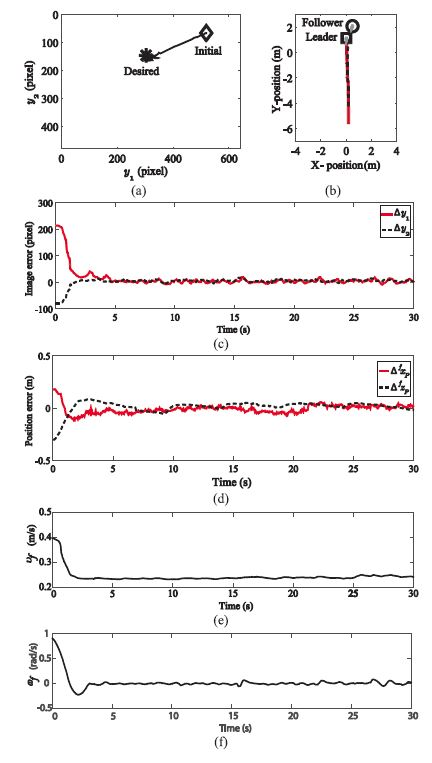
\includegraphics[width=0.6\textwidth]{figs/result1.jpg}% 1\linewidth
  \caption{Control block diagram.}
  \label{result1}
\end{figure}

\begin{figure}
  \centering
  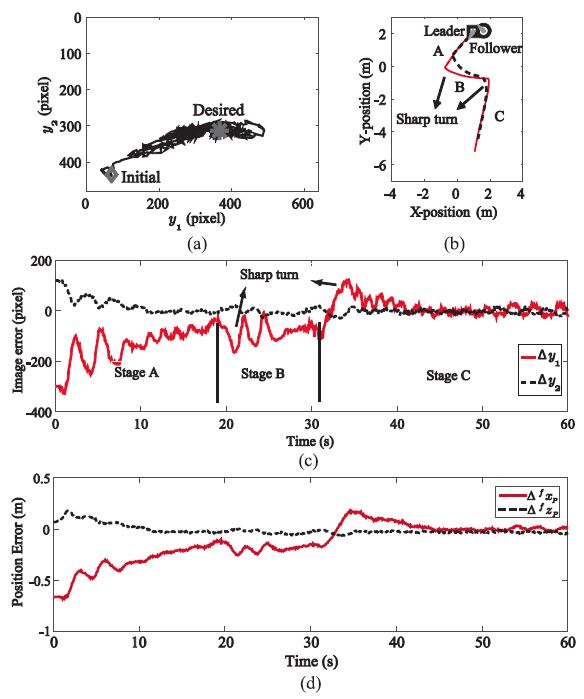
\includegraphics[width=0.6\textwidth]{figs/result2.jpg}% 1\linewidth
  \caption{Control block diagram.}
  \label{result2}
\end{figure}

\section{Some Comments on the Paper}

\indent The control error is defined on the image plane. Due to the projective property, there are multiple points in the 3D space which are projected onto one point in the 3D image space. In this case, there will be multiple state hypothesis of the system when the control error converges.


%\begin{thebibliography}{99}%\scriptsize
%    \bibitem {Kerl2013} C. Kerl, J. Sturm, and D. Cremers, “Dense visual SLAM for RGB-D cameras,” in Proc. of IEEE/RSJ Int. Conf. on Intelligent Robot Systems (IROS), 2013.
%    \bibitem {Newcombe} R. A. Newcombe, S. Izadi, O. Hilliges, D. Molyneaux, D. Kim, A. J. Davison, P. Kohli, J. Shotton, S. Hodges, and A. Fitzgibbon, “KinectFusion: Real-time dense surface mapping and tracking,” in Proc. of IEEE ISMAR, 2011.
%\end{thebibliography}

\end{document} 